\documentclass[11pt,a4paper]{article}
\usepackage[text={6.5in,10in},centering,a4paper]{geometry}
\usepackage{amssymb,amsmath} % Equations
\usepackage{tabularx} % Tables
\usepackage{graphicx,color} % Graphics, Figures
\usepackage[tight,footnotesize]{subfigure}
%\usepackage{pgfgantt}           % for gantt chart
\usepackage{hyperref}

\usepackage{indentfirst}

%\usepackage[no-math]{fontspec}

\graphicspath{{figures/}} % create a director 'figures' in your local dir and all pics are kept here

\newenvironment{conditions}[1][where:]
  {#1 \begin{tabular}[t]{>{$}l<{$} @{${}={}$} l}}
  {\end{tabular}}
 
\renewcommand\familydefault{\sfdefault} % set to San Serif series

\begin{document}
\thispagestyle{empty}
\vfill
\begin{center}
%\renewcommand{\baselinestrech}{1.2}
{
\LARGE \bf
Senior Project Report 2102499 Year 2017
}
\vfill
{
\LARGE \bf
% Project title
Analysis and Design of Planar Phased Array Antenna for \\[1ex]
5 GHz Applications
}
\vfill
{\Large \bf Norawit Nangsue ID 5730289021}  \\[2ex]
{\Large \bf Advisor: Assist. Prof. Tuptim Angkaew}
\vfill
{\Large \bf Department of Electrical Engineering }\\ [2ex]
{\Large \bf Faculty of Engineering} \\ [2ex]
{\Large \bf Chulalongkorn University}
\end{center}
\newpage
\begin{abstract}
The purpose of this report is mainly to study on both the analysis and design of the 2x2 phased array antenna which each element of the arrays are a rectangular microstrip antenna. The phased array are analyzed with multiple phased difference in order to understand the phased array behavior.  A comparison between the physical and the simulation model is included.   

\end{abstract}

\paragraph{\textbf Keywords:} phased array, microstrip, array antenna \\

%\paragraph{\textbf Remark:} A report should not have more than 25 pages (exclude Appendices and References)

% Note: the abstract should be fit in the cover

\newpage
\tableofcontents


\newpage
\section{Introduction}

The recent advances of technologies would not have happened without communication systems. Today, wireless communication is available almost everywhere in the world. One of the most important things in communication systems is the antenna, because it is able to radiate or receive radio and television transmission signals via the use the earth’s atmosphere. With these abilities, we may use it to send or receive the information that we want to instantly and cheaply. As we know, just a wire could technically be used as an antenna. However, its properties may not be good for every requirement or application.

	The freedom of using frequency bands bring us to the world of technology. Back in 1947 at the International Telecommunications Conference of the ITU  (International Telecommunication Union) in Atlantic City the first ISM (Industrial, Scientific and Medical) bands were established, which allowed us to use individual frequencies without asking for permission. For example, the microwave oven, we never have to ask for any government's permission to use microwaves which radiate the electromagnetic wave at the frequency of 2.45 GHz to our food because this  frequency is in the ISM bands.

	There are many methods to increase the range of an antenna, the easiest one is to increase the power. However, if we just want to send a message from one station to another there will be a huge power loss to the air in directions that we do not really need to transmit. A good practical engineer designs antennas that have the property of focusing in only one direction which is called Directivity. Therefore, a high directivity antenna can be able to send the signal greater distances than a non-high directivity antenna.

    Considering a water droplet dropping onto the surface of water, there will be a circular wave spreading out from the origin.  If there are multiple droplets in a row, those wave will be constructed and destructed depending on the location and it will reform like a seacoast wave. So this will make a more powerful wave from two sources. Moreover, the direction can also be changed by controlling how the droplets fall onto the surface. The same as an array of antennas, if we can control each  element's phase we will be able to control antenna's directivity as desired. 

    If we want to make a device that everyone agrees to carry everywhere they go, basically, it must be small, thin and cheap. To response to this demand, there is a flat composite material which is composed of woven fiberglass cloth available on the market, it is termed FR4 (a grade designation assigned to glass-reinforced epoxy laminate sheets, tubes, rods and printed circuit boards).
            Engineers usually uses FR4 as a micro-strip. It can be used in any type of microwave circuit including antennas.

    Therefore, there are a lot of constraints depending on which application we want use. As from the title of this proposal,  Analysis and Design of Planar Phased Array Antenna for 5 GHz Applications, this project consists of reviewing past literature, derived formula, empirical formula and try to using all of this knowledge to design an array of antenna with phase-control at the ISM band (5.8 GHz).

\newpage

\section{Project Overview}
\subsection{Objectives}
The main objectives of this project is to study about the analysis and design of the microstrip phased array with the variety of phase difference and the gain improvement when the number of patches are increased from a single patch to 2 patches and 2 patches to 4 patches. Comparing the theory models, simulation models and the physical model altogether.
\subsection{Scope of Work}
\begin{itemize}
	\item Study the design and the analysis of microstrip and phased array theory
	\item Design the antennas and microstrip transmission line
	\item Simulate the antennas and fine tune to get the better S11
    \item Shift microstrip array antenna with some phase
	\item Order the printed antenna
    \item Test the antennas
	\item Compare the antenna results with the analysis method
\end{itemize}
\subsection{Expected Outcomes}
\begin{itemize}
	\item PCB files of all designed antennas
	\item Simulation results
    \item Measurement results
\end{itemize}

\newpage

\section{Methodology}
\subsection{Microstrip Antenna}
\subsubsection{Fringing Effect}

Fringing effect causes an extra length of the microstrip patch. Therefore, a length subtraction will be required at the process of calculating the length of the patch\cite{CoB:05}

\begin{figure}[ht]
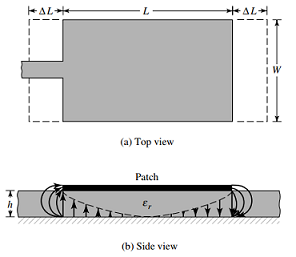
\includegraphics{fringingeffect.png}
\centering
\caption{The fringing effect that cause an extra length (adapted from )}
\end{figure}

Electric field spreading at both sides of the edges causes to adding the extra length followed as this expression\cite{CoB:05}

\begin{equation} \label{eq:fringing}
\frac{\Delta l}{h}=0.412\frac{(\epsilon_{r(eff)}+0.3)(\frac{W}{h} + 0.264)}{(\epsilon_{r(eff)}-0.258)(\frac{W}{h} + 0.8)}
\end{equation}

\begin{conditions}
 \Delta l    	 	&	Extra length of the patch \\
 		h     		&	Substrate thickness \\   
 \epsilon_{r(eff)} 	&	Effective relative dielective constant(See Appendix) \\
 		W			&	Width of the patch
\end{conditions}

\subsubsection{Preliminary Dimension}

With a given frequency, the dimension of microstrip patch can be easily designed with these expressions\cite{CoB:05,NoK:05}.
\begin{equation}
	L = \frac{c}{2f_{r}\sqrt{\epsilon_r\mu_r}} - 2\Delta l
\end{equation}
\begin{equation}
    W = \frac{c}{2f_{r}}\sqrt{\frac{2}{\epsilon_{r} + 1}}
\end{equation}

\begin{conditions}
 		L    	 	&	Length of the patch \\
        W    	 	&	Width of the patch \\
 		c     		&	Speed of light \\   
 		f_{r} 		&	Resonant frequency \\
 		\epsilon_{r}&	Relative dielective constant of the substrate \\
        \mu_{r}		&	Magnetic permeability of the substrate \\
        \Delta l    &	Extra length of the patch \\
\end{conditions}

\subsubsection{Input Impedance}

According to the transmission line model, there are 2 edges(slots) and the transmission line wire them as a parallel circuit. The derivation from cavity model represents both slots as admittance $Y$ but the transmission line model represents the transmission line as characteristic admittance.\cite{CoB:05} Howsoever, the characteristic impedance may not need to be considered because the when we rotate the smith chart at around $\frac{\lambda_g}{2}$, the smith chart will be around at the same point.\newline

\begin{figure}[ht]
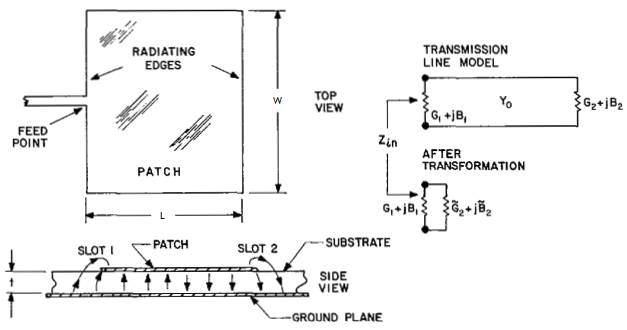
\includegraphics{tlmodel.png}
\centering
\caption{Transmission line model (adapted from \cite{CaM:81})}
\end{figure}

The slot admittance can be represent as $Y_1 = G_1 + jB_1$. As mentioned before, $G_1$, slot conductance, expressed by the cavity model is\cite{CoB:05}
\begin{equation}
    G_1 = \frac{2P_{rad}}{|V_0|^2}=\frac{I_{1}}{120\pi^2}
\end{equation}
\begin{equation}
    I_1 = \int_{0}^{\pi} \left[\frac{\sin\left(\frac{X}{2}\cos{\theta}\right)}{\cos{\theta}}\right]^2 \sin^3{\theta} d\theta = -2 + \cos(X) + XS_i(X) + \frac{\sin(X)}{X} 
\end{equation}
\begin{equation}
X = k_0W
\end{equation}

by
\begin{equation}
	P_{rad} = \frac{|V_0|^2}{2\pi\eta_0} \int_{0}^{\pi} \left[\frac{\sin\left(\frac{X}{2}\cos{\theta}\right)}{\cos{\theta}}\right]^2 \sin^3{\theta} d\theta
\end{equation}

\begin{conditions}
 		G_1    	 	&	Slot conductance \\
        P_{rad}    	&	Radiation power \\
 		V_0     	&	Input voltage \\   
 		k_0			&	Wavenumber \\
 		\eta_0		&	Impedance of free space\\
        Si(x)		&	Sine integral(See Appendix)\\
\end{conditions}

\newpage
The component $B_1$ could be neglected if the slot distance is separated by the distance around $\frac{\lambda_g}{2}$ which caused $B_2 \approx -B_1$. But for $G_2$, due to the slots have almost the same width, then its value is the same to $G_1$ and it could be also written as $G_2 \approx G_1$. Therefore, the total admittance would be
\begin{equation}
Y_{in} = Y_1 + Y_2 = G_1 + jB_1 + G_2 - jB_2 \approx 2G_1
\end{equation}

And, the input impedance is surely be

\begin{equation}
Z_{in} = \frac{1}{Y_{in}} = \frac{1}{2G_1}
\end{equation}

However, this equation doesn't take mutual effects into account. So, $G_{12}$ is introduced as a mutual conductance and the impedance equation must be altered to\cite{CoB:05}

\begin{equation}
Z_{in} = \frac{1}{2(G_1 \pm G_{12})}
\end{equation}

by
\begin{equation}
G_{12} = \frac{1}{|V_0|^2}\textrm{Re}\int\int_{S}\vec{E_1} \times \vec{H^*_2} \cdot d\vec{s} = \frac{1}{120\pi^2} \int_{0}^{\pi} \left[\frac{\sin\left(\frac{X}{2}\cos{\theta}\right)}{\cos{\theta}}\right]^2 J_0(Y\sin{\theta}) \sin^3{\theta} d\theta
\end{equation}

\begin{equation}
X = k_0W
\end{equation}
\begin{equation}
Y = k_0L
\end{equation}

\begin{conditions}
 		G_{12}   	&	Mutual conductance \\
        V_0			&	Input voltage \\
        \vec{E_1}   &	Electric field radiated by the slot \#1\\
 		\vec{H_2} 	&	Magnetic field radiated by the slot \#2\\
 		\vec{s}		&	Area vector\\
		J_0			&	Zero order Bessel function \\ 
        k_0			&	Wavenumber \\
 		W			&	Width of the patch\\
        L			&	Length of the patch\\
\end{conditions}

\subsubsection{Matching Technique}
There are many several technique to perform matching a single microstrip patch antenna such as\cite{AtT}
\begin{itemize}
	\item Quarter Wave Impedance Transformer (See appendix)
    \item Inset Feed
    \item Coupled(Indirect) Feed
    \item Aperture Feed
    \item Coaxial Feed
\end{itemize}

In this project, quarter wave impedance transformer will be used because this technique is the most basic one and the patch will not be suffered from trimming at the feed point. Consequently, it's more versatile to build an array antenna comparing to the coaxial feed. 

\subsubsection{Radiation Pattern}
%add image and more text
Derived from the cavity model\cite{NkN:16}, at $TM_{010}$ mode, the radiation field is
\begin{equation}
        E_{\phi} = j\frac{k_0WV_0}{\pi r}e^{-jk_0r} \left(\cos\theta \sin\phi \frac{\sin{X}}{X}\frac{\sin{Y}}{Y}\right) \times \cos(Z)
\end{equation}
\begin{equation}
        E_{\theta} = j\frac{k_0WV_0}{\pi r}e^{-jk_0r} \left(\cos\phi \frac{\sin{X}}{X}\frac{\sin{Y}}{Y}\right) \times \cos(Z)
\end{equation}

\begin{equation}
        f(\theta,\phi) = \sqrt{\vec{E^2_\phi} + \vec{E^2_\theta}} = \sqrt{1 - \sin^2{\phi}\sin^2{\theta}} \cdot \frac{\sin{X}}{X}\frac{\sin{Y}}{Y}\cos{Z}
\end{equation}

by

\begin{equation}
        X = \frac{k_0 h}{2} \sin{\theta} \cos{\phi}
\end{equation}

\begin{equation}
        Y = \frac{k_0 W}{2} \sin{\theta} \cos{\phi}
\end{equation}

\begin{equation}
        Z = \frac{k_0 L_{eff}}{2} \cos{\theta}
\end{equation}



\begin{conditions}
%Fix
 		E_{\phi}   	&	Electric field at coordinate \\
        E_{\theta}  &	Electric field at coordinate \\
        f_{\theta,\phi} & Normalized field pattern\\
        k_0			&	Wavenumber \\
 		W			&	Width of the patch\\
        L			&	Length of the patch\\
\end{conditions}
      

\subsubsection{Design Procedure}

\subsection{Array Theory}
\subsection{Microstrip Network}
\subsection{Power Divider}
\subsection{Microstrip Array Antenna}
\subsubsection{1x2 Array Antenna}
\subsubsection{1x2 Array Design Procedure}
\subsubsection{2x2 Array Antenna}
\subsubsection{2x2 Array Design Procedure}
\subsection{Phase Shift by Translating Feed Point}
\subsubsection{1x2 Array Antenna with 180 degree phase different}


\section{Results}
%Computer Calculation, Computer Simulation, Physical Measurement

\section{Discussion}
\subsection{Affect on the Ground Plane}
\subsection{Array Factor Usage}
\subsection{Undesired lobes}

\section{Conclusions}

\section{Acknowledgement}
(optional)


\subsection{References}
Reference formats are different from reference types. We commonly use the IEEE format, found in 

\url{https://www.ieee.org/documents/ieeecitationref.pdf}

Use BibTex to generate reference list in the document. You will need a list of reference in the format of \texttt{file.bib} containing reference details, which can be exported easily using Google Scholar. When to refer to a paper, use \texttt{cite}. For example, the concept about system identification can be read from~\cite{SoS:89}.

\bibliography{ref}
\bibliographystyle{plain}

% Appendix Section
\section{Appendices}
\subsection{Effective Dielectric Constant of Microstrip}

\subsection{Sine Integral, Si(x)}

\subsection{Quarter Wave Impedance Transformer}

\subsection{Hammerstad's Microstrip Characteristic Impedance Synthesis Equation}

\subsection{Effective Relative Dielective Constant Equation}

\subsection{Mitered Microstrip Bends}

\end{document}
